\documentclass[tikz]{standalone}


\usepackage{tikz}
\usetikzlibrary{calc}

\begin{document}
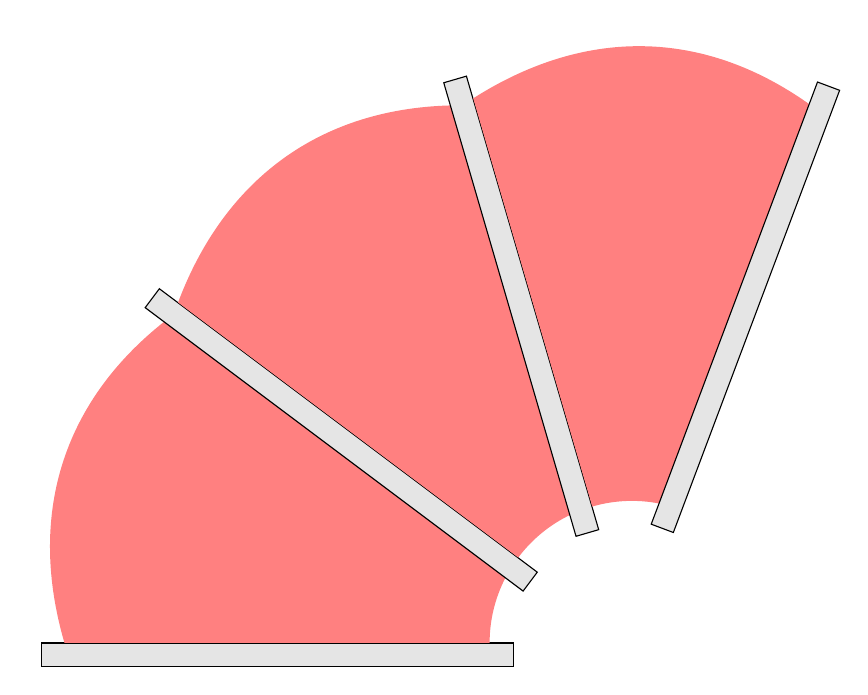
\begin{tikzpicture}[
	scale=3,
	plate/.style={draw, fill=gray!20},
	rubber/.style={fill=red!50}
]


\def\h{.1} 	% height of plate
\def\l{2}	% length of plate
\def\x{.5}	% distance of Rotation point
\def\extradist{.2}
\def\n{3}	% number of plates
\def\xr{.05} % relative distance of rubber from plate ends


\pgfmathsetmacro{\dalp}{asin((\h+\extradist)/(\x))}
\pgfmathsetmacro{\dbet}{atan(\h/((1-\xr)*\l+\x))}
\pgfmathsetmacro{\dgam}{atan(\h/(\xr*\l+\x))}
\pgfmathsetmacro{\xrinv}{1-\xr}
\pgfmathsetmacro{\xrinvbar}{1-2*\xr}


\foreach \i in {0, ..., \n}{
	\pgfmathsetmacro{\alp}{\i*\dalp}
	\path (180-\alp:\x)--++(180-\alp:\l)--++(270-\alp:\h)--++(-\alp:\l)coordinate[pos=\xr](L);
	\ifnum\i>0
		\path (L)arc(180-\alp+\dbet:180-\alp+\dalp:\x+\xrinv*\l)coordinate(LL);
		\path[rubber] (L)to[out=-\alp-90-\dalp*.4, in=-\alp-\dalp+180](LL)--++
		(-\alp+\dalp:\xrinvbar*\l)arc(180-\alp+\dalp:180-\alp+\dgam:\x+\xr*\l)--cycle;
	\fi
	\path[plate] (180-\alp:\x)--++(180-\alp:\l)--++(270-\alp:\h)--++(-\alp:\l)--cycle;
}


\end{tikzpicture}
\end{document}